\documentclass[../mathNotesPreamble]{subfiles}

\providecommand{\relscalefact}{1.4}
\begin{document}
\relscale{\relscalefact}
  \section{1.6: Absolute Value Functions}

  \begin{defn*}[Absolute Value Function]
    The absolute value function can be defined as a piecewise function
      \[f(x)=\abs{x}=
      \begin{cases}
        \phantom{-}x, &\textnormal{ if } x\geq 0\\
        -x, &\textnormal{ if } x<0
      \end{cases}\]
  \end{defn*}
  \begin{ex*}
    Graph the following
    \begin{extasks}[after-item-skip=\stretch{1}](2)
      \task 
        $f(x)=\abs{x}$
        \begin{center}
          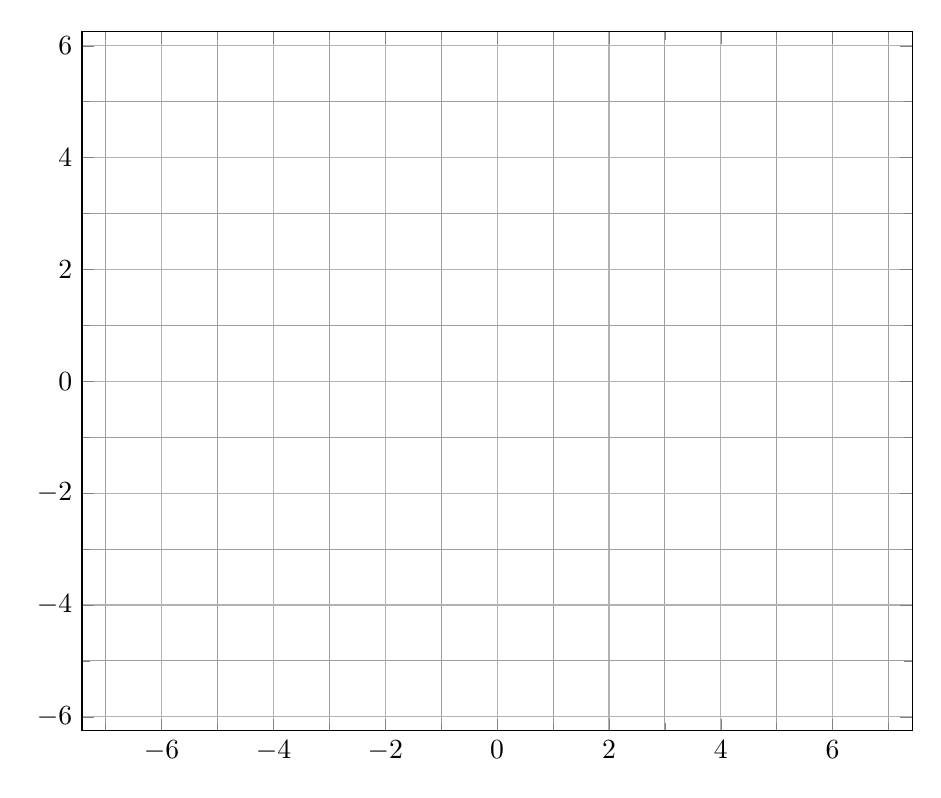
\begin{tikzpicture}[declare function={
            f(\x)=sqrt(4-x^2);
            }]
            \begin{axis}[
                grid=both, %major,minor
                grid style={line width=0.375pt, draw=gray!60},
                axis equal,
                minor grid style={draw=gray!75},
                xmin=-6, xmax=6,
                ymin=-6.25, ymax=6.25,
                width=\linewidth,
                minor x tick num=1,
                minor y tick num=1,
                xlabel=, ylabel=,
                xtick={-8,-6,...,8},
                ytick={-8,-6,...,8}
                ]
            \end{axis}
          \end{tikzpicture}
        \end{center}
      \task 
        $f(x)=\abs{x-2}$
        \begin{center}
          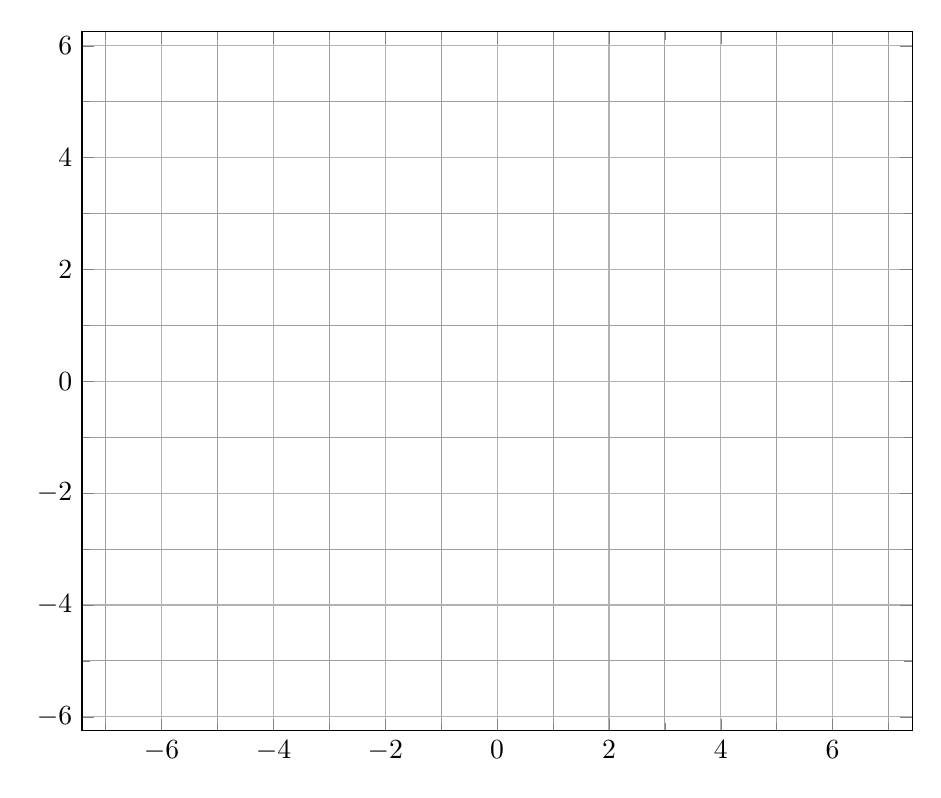
\begin{tikzpicture}[declare function={
            f(\x)=sqrt(4-x^2);
            }]
            \begin{axis}[
                grid=both, %major,minor
                grid style={line width=0.375pt, draw=gray!60},
                axis equal,
                minor grid style={draw=gray!75},
                xmin=-6, xmax=6,
                ymin=-6.25, ymax=6.25,
                width=\linewidth,
                minor x tick num=1,
                minor y tick num=1,
                xlabel=, ylabel=,
                xtick={-8,-6,...,8},
                ytick={-8,-6,...,8}
                ]
            \end{axis}
          \end{tikzpicture}
        \end{center}
      \task 
        $f(x)=\abs{x}+3$
        \begin{center}
          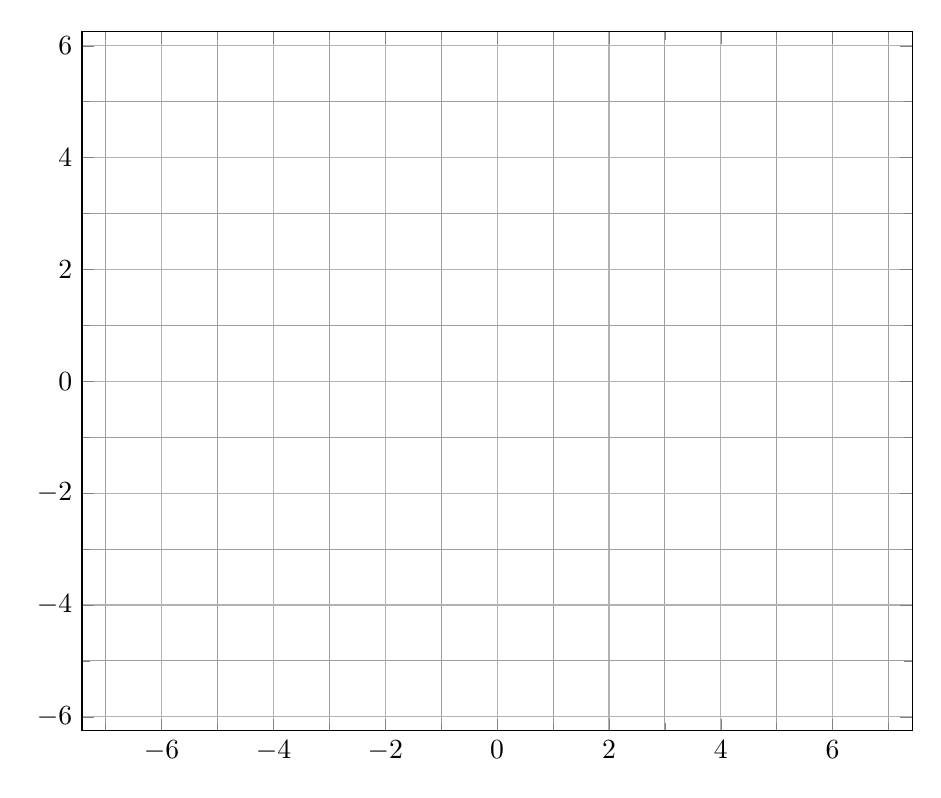
\begin{tikzpicture}[declare function={
            f(\x)=sqrt(4-x^2);
            }]
            \begin{axis}[
                grid=both, %major,minor
                grid style={line width=0.375pt, draw=gray!60},
                axis equal,
                minor grid style={draw=gray!75},
                xmin=-6, xmax=6,
                ymin=-6.25, ymax=6.25,
                width=\linewidth,
                minor x tick num=1,
                minor y tick num=1,
                xlabel=, ylabel=,
                xtick={-8,-6,...,8},
                ytick={-8,-6,...,8}
                ]
            \end{axis}
          \end{tikzpicture}
        \end{center}
      \task 
        $f(x)=2\abs{x-3}+1$
        \begin{center}
          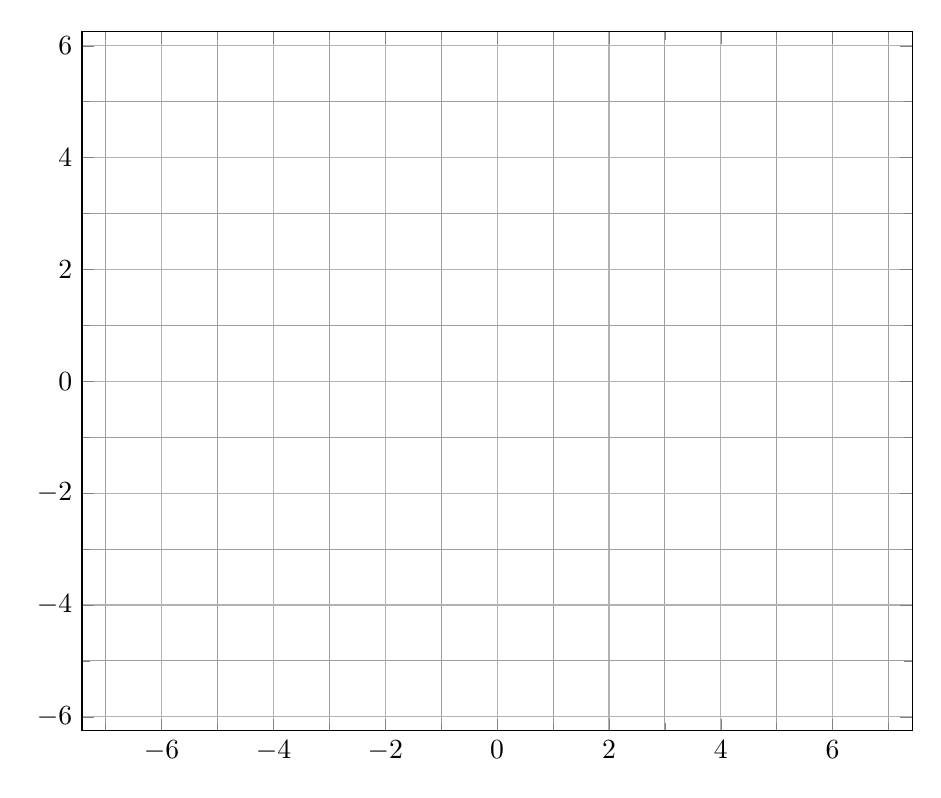
\begin{tikzpicture}[declare function={
            f(\x)=sqrt(4-x^2);
            }]
            \begin{axis}[
                grid=both, %major,minor
                grid style={line width=0.375pt, draw=gray!60},
                axis equal,
                minor grid style={draw=gray!75},
                xmin=-6, xmax=6,
                ymin=-6.25, ymax=6.25,
                width=\linewidth,
                minor x tick num=1,
                minor y tick num=1,
                xlabel=, ylabel=,
                xtick={-8,-6,...,8},
                ytick={-8,-6,...,8}
                ]
            \end{axis}
          \end{tikzpicture}
        \end{center}
    \end{extasks}
    \vspace*{\stretch{1}}
  \end{ex*}
  \pagebreak

  \begin{ex*}
    Solve the following equations
    \hspace*{\stretch{1}}
    \textcolor{blue}{\underline{\href{https://www.desmos.com/calculator/ge2qz4yl2m}{Graphs}}}
    \begin{extasks}[after-item-skip=\stretch{1}](2)
      \task $\abs{x}=3$
      \task $\abs{2x+6}=2$
      \task $\abs{x+3}-1=0$
      \task $2-\abs{4-x}=0$
    \end{extasks}
    \vspace*{\stretch{1}}
  \end{ex*}
  \pagebreak
  \begin{ex*}
    Solve the following inequalities
    \hspace*{\stretch{1}}
    \textcolor{blue}{\underline{\href{https://www.desmos.com/calculator/7xusrxlcas}{Graphs}}}
    \begin{extasks}[after-item-skip=\stretch{1}](2)
      \task $\abs{x-5}\leq 4$
      \task $\abs{\dfrac{x}{4}-1}<2$
      \task $\abs{2-x}\leq 3$
      \task $\abs{x-3}>2$
    \end{extasks}
    \vspace*{\stretch{1}}
  \end{ex*}
  \pagebreak

\end{document}
